%!TEX root = ../../report.tex
\chapter{Conception and initial analysis} % (fold)
\label{cha:analysis}
The process of sketching a bipedal robot as the presented here implies that the essential variables for the design have to be identified and determined aiming at the most optimal solution possible\footnote{Optimality here is measured in terms of the aimed goals, described in \ref{sec:goals}.}.
The important role of the geometrical and inertial mechanical parameters in locomotion control was first proved by \cite{passive_walking}, and their relevance deserves a careful study.
Hence, the sections in this chapter contain the conceptual presentation of a set of design criteria and the first approaches to the construction of the RuBi prototype arisen from the study of these parameters and the application of these criteria.

%!TEX root= ../../../report.tex

\section{Bipedal locomotion} % (fold)
\label{sec:bipedal_walking_and_running_gaits}
This section contains a superficial comparative study of the characteristics of human-like walking and running patterns.
The reason is to help justify in the following chapters the decisions taken during the design.

Although walking and running motion patterns in humans might resemble each other at first glance, they contain important variations that imply that a robot able to walk at a certain speed is not necessary capable of running at the same speed, or running at all.
The existence of the so-called "flight phase" in running but not in walking cycles is the main difference between them.
This phase encompasses the period in which there is no contact between the feet and the ground and causes the main variations in energy and trajectory generation.

\subsection{Walking and running gaits comparison} % (fold)
\label{sub:walk_and_run_comparison}
The differences in both joint kinematics and kinetics between both patterns arisen from this distinction are studied in \cite{grimmer}, Manuscript I, for a wide range of speeds.
From the cited paper it can be seen that the joint positions for a whole cycle in both walking and running patterns are very similar, specially for hip and knee.
Furthermore, the joint velocity profiles have almost the same shape but differ in the magnitudes, being higher the angular speeds reached for running.
Similar conclusions can be extracted from a quick comparison between the torque and power profiles in a running and walking cycle.
While the shapes of the functions for the three joints are the really close, with bigger differences for the ankle, the values of the curve are in average smaller for human walking than for running.
As expected, the conclusion is that higher requirements for joint speed, torque and power are expected for running, specially for the knees and the ankles.

% Impact forces comparison here
Besides, the foot strike and impact forces during the landing phase in both cases change, both in intensity and profile. ***

% subsection walk_and_run_comparison (end)

% section bipedal_walking_and_running_gaits (end)
%!TEX root = ../../../report.tex

\section{Geometrical dimensions of the frame} % (fold)
\label{sec:dimensions}
The selection of the final dimensions of RuBi corresponds to an iterative process in which power requirements and achieving human-like kinematics have been the main constraints when assessing the size of the robot.
A first approach was taken from \cite{grimmer}, Manuscript I, where normalized values of power required per joint and per kilogram of the structure can be found.
The first iteration targeted a robot of dimensions $m = 1Kg$ and length from the hip joint to the tip toes of $L = 0.6 m$ for a fully stretched leg.
The final parameters from the last iteration can be found in ***%***chapter Results

Once estimated an overall length of the structure, an initial value of the dimensions of each link were decided to be obtained based on the German section of the ISO 7250-2 \cite{iso_measurements} and the DIN 33402-2 \cite{din_measurements1} norms, following the idea of mimicking human-like motion as closely as possible.
These two norms are standard references in industry and were considered a general enough source of information.
Figure \ref{fig:human_measurements} depicts some of the human dimensions extracted from the norms and applied to the design of RuBi.
Their names and values for male between 18-65 year old and in percentile 50 can be found in table \ref{tab:din_proportions}.

\begin{figure}[h]
	\centering
	\begin{subfigure}[b]{0.3\textwidth}
        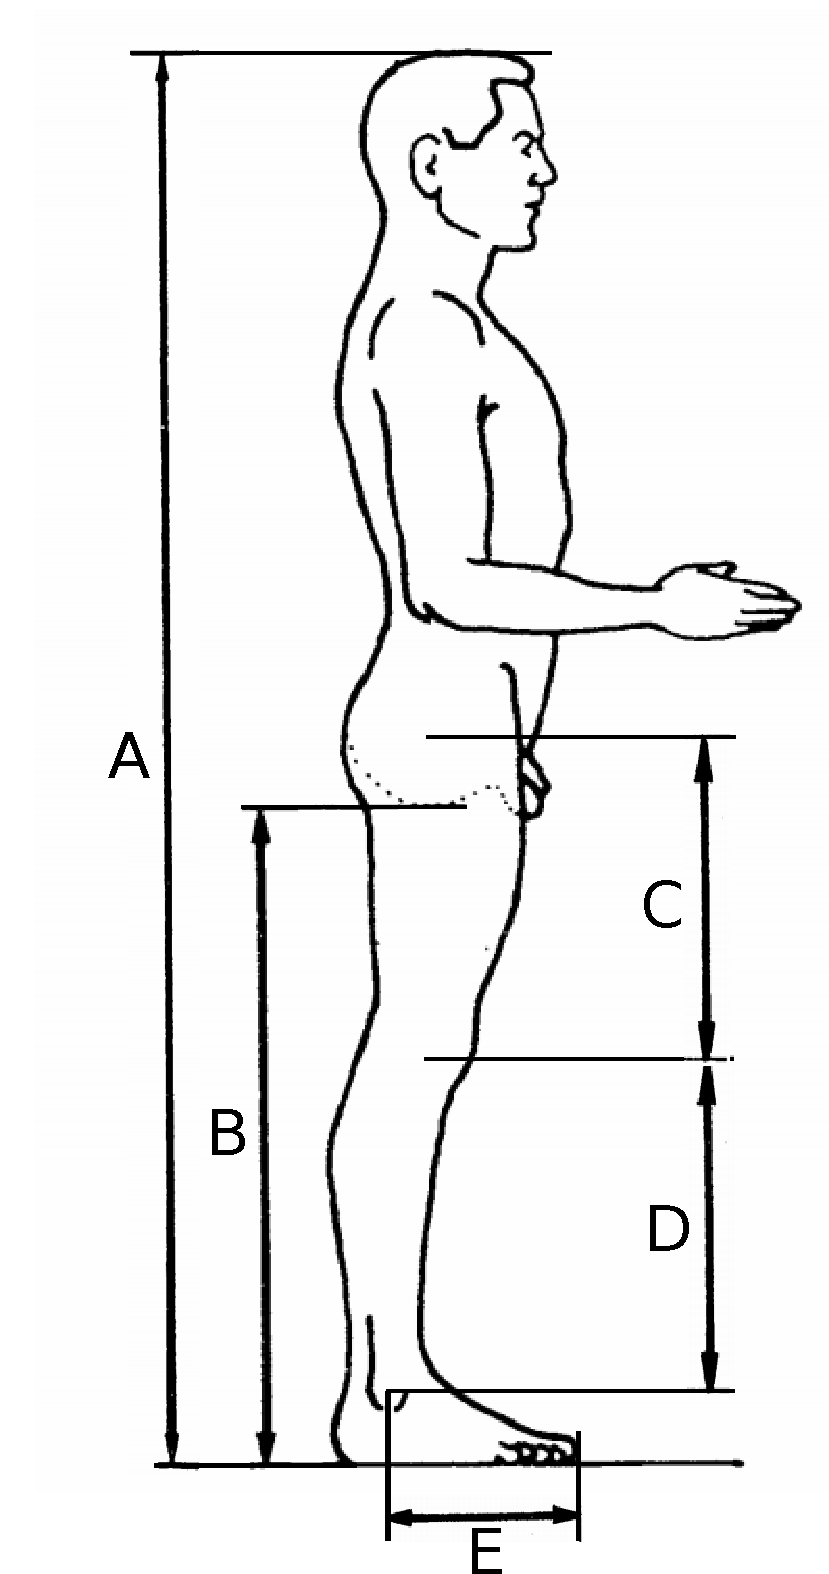
\includegraphics[width=\textwidth]{figures/din_measurements.pdf}
        \caption{Left foot}
        \label{fig:din1}
    \end{subfigure}
    \begin{subfigure}[b]{0.4\textwidth}
        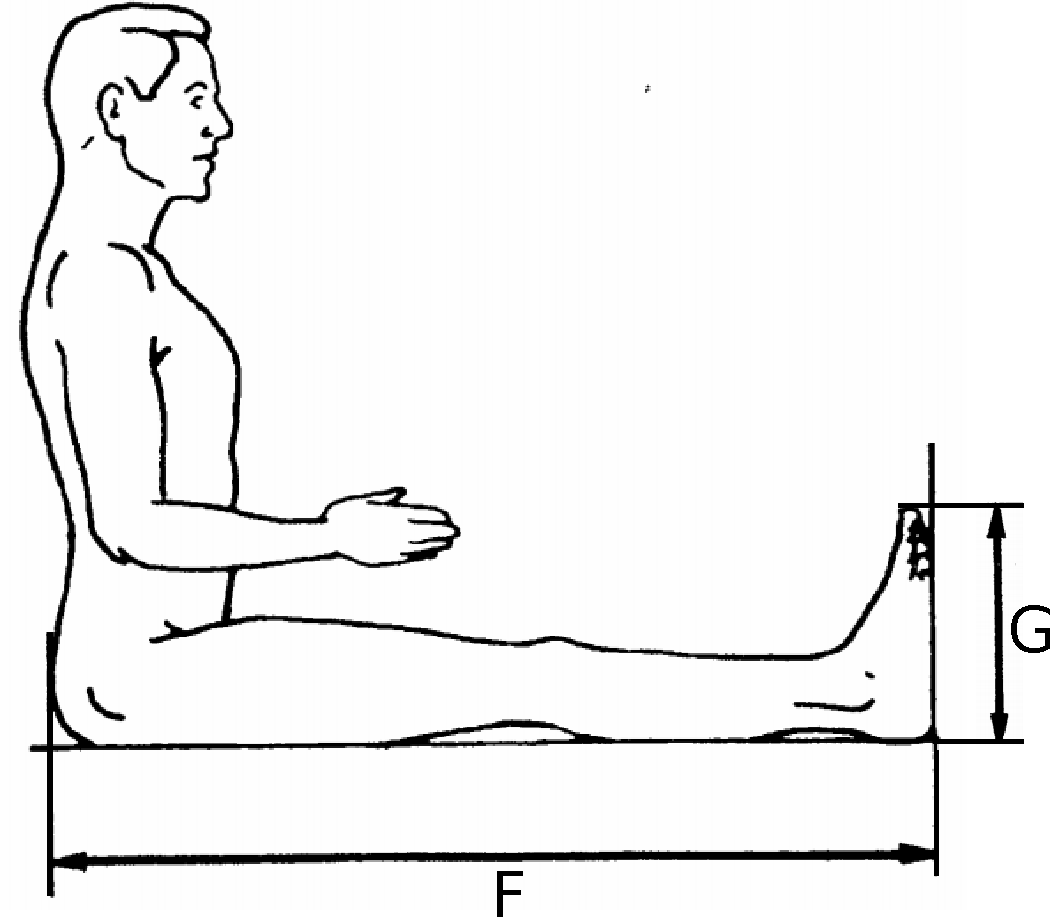
\includegraphics[width=\textwidth]{figures/din_measurements2.pdf}
        \caption{Hip}
        \label{fig:din2}
    \end{subfigure}
	\caption{Lower body measurements used for RuBi. Picture adapted from \cite{din_measurements1}.}
	\label{fig:human_measurements}
\end{figure}


\begin{table}
\begin{center}
	\begin{tabular}{c | c | c | c}
	  Index & Definition & Value & \% of Stature \\
	  \hline
	  A & Stature (body height) & ** & 100 \\
	  B & Crotch height & ** & ** \\
	  C & Femur height & ** & ** \\
	  D & Tibial height & Not in norm & **\\
	  E & Ankle-toe tip distance & Not in norm & ** \\
	  F & Buttocks-leg length & ** & ** \\
	  G & Sole length & ** & **
	\end{tabular}
	\caption{Human proportions from DIN 33402-2}
	\label{tab:din_proportions}
\end{center}
\end{table}

\subsection{Limbs length} % (fold)
\label{sub:limbs_lengths}
The dimensions needed to create a simplified model of one leg are the limbs lengths, which are the straight line distances measured from two consecutive joints.
They have been called $l_{i}$ where $i$ is the robot link + joint as per table \ref{tab:limb_index} and can be seen in Figure \ref{fig:kinematics}.
However, the norm does not determine all of them.

\begin{table}
\begin{center}
	\begin{tabular}{c | c | c}
	  $l_{i}$ & Limb \\
	  \hline
	  $l_{1}$ & Hip + thigh & C \\
	  $l_{2}$ & Knee + Foreleg & D\\
	  $l_{3}$ & Ankle + foot & E 
	\end{tabular}
	\caption{Limbs index}
	\label{tab:limb_index}
\end{center}
\end{table}

Since $C$ and $E$ are not standard measurements in industry, they have been obtained as follows:

\paragraph{The Femur height}
The crotch height, denoted as $B$ in the figure, has been averaged with the buttocks-leg length and the tibial height + an empirical approximation of the height of the ankle have been subtracted from the result, obtaining $C$.

\paragraph{The ankle-toe tip distance}
Since this distance is not standard either, it has been obtained once again adjusting the sole length with empirical measurements.
% subsection limbs_lengths (end)

\subsection{Hip and sole width} % (fold)
\label{sub:subsection_name}
The hip width sitting, as defined in the norm and for the same sample group than before, has been used as starting point to define the final width of the structure of the hip.
This standard measurement has been scaled down to a human of length L from hip joint to toe tip, which would correspond to $L=C+D+E$, using the proportion between stature and lower body lengths, also obtained from the norm.
The same process has been conducted to calculate the implemented width of the foot sole.

% subsection hip_sole_width (end)

No other standard measurement has been used as reference for the design, such as thigh or lower leg circumferences, since they do not affect the kinematics of the structure although they have a big influence in its dynamics.
The criteria followed to model the dynamics of the robot is explained in \ref{sec:physical_properties}.


%% Here we just describe the process followed to obtain the final dimensions. 
%% The final results are shown in Chapter Results --> add tables and Froude number calculus


% section dimensions (end)
%!TEX root = ../../../report.tex

\section{Inertial dimensions of the frame} % (fold)
\label{sec:physical_properties}
This section presents the theoretical guidelines followed during the design of RuBi regarding its dynamic model.
The calculations carried out are to be found in chapters \ref{cha:mathematical_model} and \ref{cha:design}. 
The determination of the geometrical dimensions for a robot model is in general a deterministic task in which all the parameters can be selected without dependencies or limitations.
However the inertial parameters of a robot will be the result of the selection of these dimensions, together with the materials utilized for the implementation and the configuration of the elements on the structure, among others.
Here, the goal of the adjustment of the final inertial parameters is not to mimic the dynamics of human legs as with the kinematics, but to reduce the power requirements for locomotion while ensuring robustness and reliability.
The main inertial parameters object of study here are the mass of the links, the positions of their CoM and their inertia moments.
Other parameters with an influence in the model dynamics such as frictions or delays introduced by transmissions are not discussed here due to the complexity of its determination at this stage of the project.

\subsection{Mass of the limbs} % (fold)
\label{sub:mass_of_the_limbs}
The mass of each limb $i$ will depend on the materials used, their geometry and their density together with any other component added to the link (actuators, electronics, transmissions).
As explained before, keeping the overall mass of the frame as low as possible while guaranteeing the fulfillment of all the structural requirements such as resistance and resilience has been one of the main goals of the analyses conducted in the design of RuBi.
This criteria led to the allocation of the embedded electronics off the robot and aim at small electric actuators as the lightest possible solution for the actuation. 
The calculations to select the limb material and profile are to be found in \ref{sub:limb_profile}.
The final masses per limb have been obtained as an approximate sum of the components that constitute them, due to the complexity of measuring them directly or using system identification techniques. 
They can be seen in %\ref{} reference to Results table and Implementation section
And they have been assumed to be concentrated in the CoM of each link for the computation of the dynamic model.
% subsection mass_of_the_limbs (end) 

\subsection{Centers of mass} % (fold)
\label{sub:centers_of_mass}

\paragraph{Limbs center of mass} % (fold)
\label{par:limbs_center_of_mass}
Limbs center of mass
The position of the center of mass of each limb referred to its joint rotational axis is a function of its masses, their distributions and its geometry.
Their coordinates are given referred to a local reference frame attached to each joint, with its $Z$ axis perpendicular to the sagital plane and its $X$ and $Y$ axes parallel to its equivalents in the main reference frame in the hip, shown in Figure \ref{fig:kinematics}.
Its direct influence in the dynamics of the system is shown in \ref{sec_dynamic_model}, equation \ref{eq:N-E_eq1}.
The coordinates of the CoM of the limbs have been estimated during the design through the 3D CAD design software tool SolidWorks \cite{solidworks}.
Their final values can be found in %\ref{} reference to Results table and Implementation section
% paragraph limbs_center_of_mass (end)

\paragraph{Center of mass of the frame} % (fold)
\label{par:center_of_mass_of_the_frame}
Frame center of mass
The location of the frame center of mass plays a very important role in the stability of the robot \cite{rojas}.
Its theoretical placement when standing still should be in the sagital plane of the structure, as close to the hip as possible, similar to humans (accounting that there is no torso).
A robust locomotion should result in a controlled and limited motion of the CoM. 
A high positioning of the CoM in the structure would make it more sensitive to the actuators influence, allowing a better balance control, while a lower placement in the structure could increase its robustness against inertial phenomenas.
The trade-off between these two criteria has been tried to be found.
As for the limbs, the coordinates of the CoM of the structure have been computed through SolidWorks and their final values can be found in %\ref{} reference to Results table and Implementation section

% paragraph center_of_mass_of_the_frame (end)
% subsection centers_of_mass (end)

\subsection{Moments of inertia} % (fold)
\label{par:moments_of_inertia}
The inertia moments of each limb will be the result of the distribution of the masses with respect to the joint axis.
Keep the CoM close to the joints to reduce them!--> smaller torque required for same angular accelerations***


% subsection moments_of_inertia (end)



%Friction model and transmissions delays not included because of its complexity

% section physical_properties (end)
%!TEX root = ../../../report.tex
\section{Joints} % (fold)
\label{sec:joints}

\begin{figure}[ht!]
  \centering
  \includegraphics[width=\textwidth]{figures/20160518_195014.jpg}
  \caption{Might help}
  \label{fig:figure1}
\end{figure}

  \subsection{Actuators} % (fold)
  \label{sub:actuators}

  %Need of angular motion for the joints: possible ways of generating it?

  % subsection actuators (end)

  \subsection{Transmission} % (fold)
  \label{sub:transmission}

  %Reduction of the moments of inertia
  %Introduction of delays and loss of accuracy 

  % subsection transmission (end)

  \subsection{Compliance} % (fold)
  \label{sub:compliance}

  %Flexible vs stiff drive train
  %Power peak and average consumption comparisons 


  \begin{figure}[hb!]
    \begin{subfigure}{.19\textwidth}
      \centering
      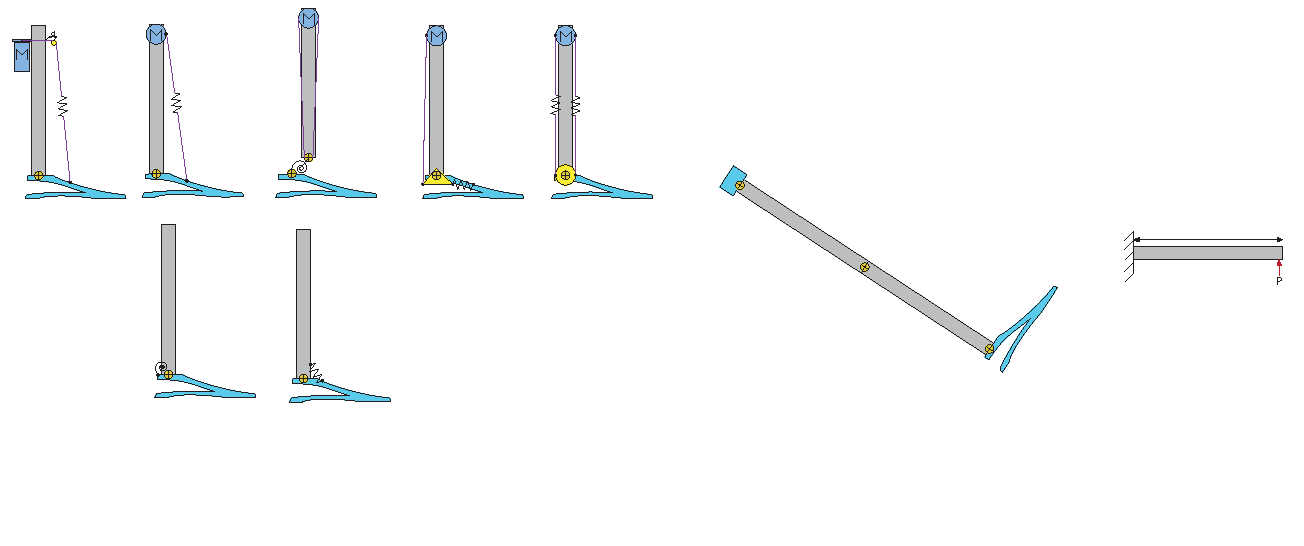
\includegraphics[width=\linewidth]{figures/illustration_serial_pulley.pdf}
      \caption{Serial pulley}
      \label{fig:series_pulley}
    \end{subfigure}
    \begin{subfigure}{.19\textwidth}
      \centering
      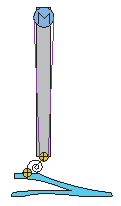
\includegraphics[width=\linewidth]{figures/illustration_serial_rotational.pdf}
      \caption{Series rotational}
      \label{fig:series_rotational}
    \end{subfigure}
    \begin{subfigure}{.19\textwidth}
      \centering
      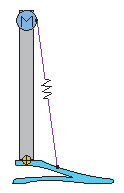
\includegraphics[width=\linewidth]{figures/illustration_serial_direct_i.pdf}
      \caption{Series direct 1}
      \label{fig:series_direct_i}
    \end{subfigure}
    \begin{subfigure}{.19\textwidth}
      \centering
      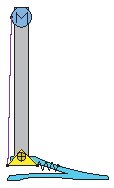
\includegraphics[width=\linewidth]{figures/illustration_serial_direct_ii.pdf}
      \caption{Series direct 2}
      \label{fig:series_direct_ii}
    \end{subfigure}
    \begin{subfigure}{.19\textwidth}
      \centering
      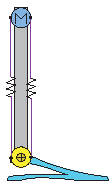
\includegraphics[width=\linewidth]{figures/illustration_serial_elastic_band.pdf}
      \caption{Series elastic band}
      \label{fig:series_elastic_band}
    \end{subfigure}
  \end{figure}  

  % subsection compliance (end)

% section joints (end)

% chapter analysis (end)